\documentclass[notitlepage]{article}
\usepackage[margin=0.75in]{geometry}
\usepackage{graphicx}
\author{Chris Manchester, Orren Saltzman}
\title{CIS 573 Project: Runtime Metamorphic Testing with Calico}
\parindent 0pt
\parskip 10pt

\begin{document}
\maketitle

\section{Introduction}

Calico is a C source code rewriter to be used to perform runtime metamorphic property testing on C programs. Calico takes as input a C source file, in which one or more functions has been annotated by the user according to a specified grammar (described below). This grammar conveys the metamorphic properties the function (or functions) is intended to have. Calico's output is a C program that behaves exactly as the original, except that each time an annotated function is called, it is called again with tranformed inputs, and the result is saved. The original output is also transformed, and it is asserted by the new program that the two results are equal. If they are, nothing has been proven about the correctness of the program, but if they are not, then the metamorphic property being asserted by the user has been violated, and the function under test has been to shown to be incorrect.

\begin{figure}[ht!]
\centering
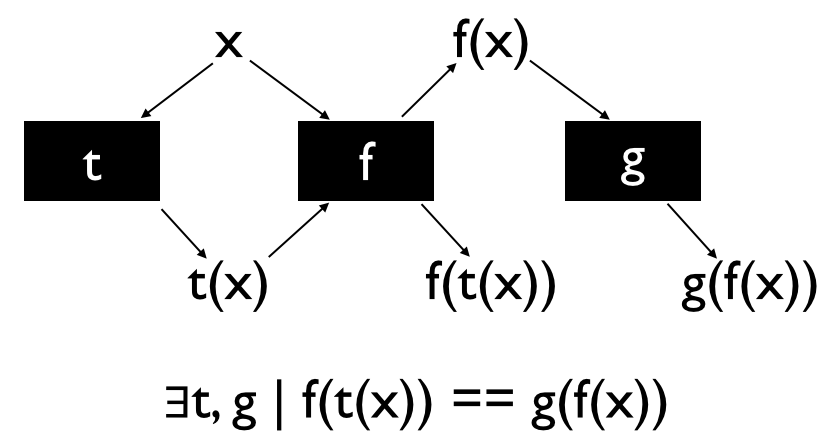
\includegraphics[width=175mm]{calico_pic1.png}
\caption{To specify a metamorphic property for the Function Under Test, f, the user must specify some functions t and g such that this equality holds.}
\end{figure}

\section{A Brief Description of Calico Instrumentation}

Many functions, particularly C functions, use side effects to accomplish their task. Furthermore, the data that might semantically be referred to as the \"result\" of a C function is not necessarily the same as the return value of that function. As such, it is necessary to assume that any piece of memory belonging to the process of the instrumented program might be considered $f(x)$ for the purpose of these assertions. Thus, it is neccessary to sandbox the effects of the function under test each time it is called, by spawning a new process for every additional time the function is called, times the number of properties being asserted. For instance, if a function is called by the application 100 times over the course of program execution, and three properties about the function are being specified, then the instrumented program must make 400 calls to the function: The original 100, plus 100 for each specified input transformation. For each of the 300 transformed calls, a process must be spawned and the result recovered through the use of shared memory. In this way, all side effects are sandboxed, and the entire application environment is held constant save the input to the function.

The form of the instrumented application is as follows:

\begin{figure}[ht!]
\centering
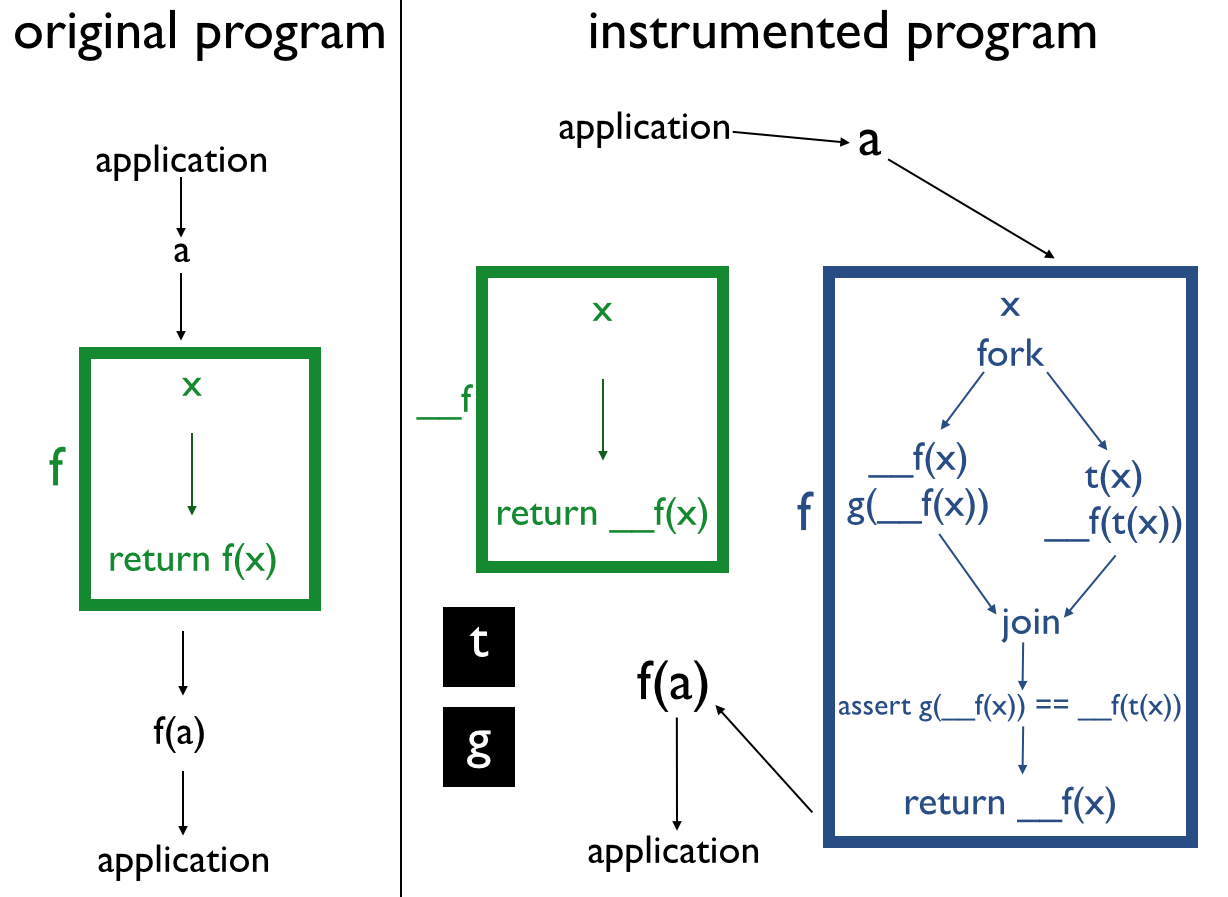
\includegraphics[width=175mm]{calico_pic2.png}
\caption{Calls to the function f are intercepted by a new function of the same name. The original is renamed with two leading underscores.}
\end{figure}

\section{The Annotation Language}

Annotations are placed in the comment text of a C function (above a function, between a /** and a */). Their form is as follows ({\bf ?} means 0 or 1 times, {\bf +} means 1 or more times, {\bf *} means 0 or more times{\bf}):

\ttfamily

<annotated-comment> ::= <unannotated-comment-text>{\bf ?} \\
\phantom{1}\hspace{120pt}<function-info-annotation> \\
\phantom{1}\hspace{120pt}<param-info-annotation>{\bf *} \\
\phantom{1}\hspace{120pt}<assertion-pair>{\bf +} \\

<function-info-annotation> ::= @fun-info { <function-name>, <function-kind>, <return-type> } ;

<function-kind> ::= PrimitiveReturn | PointerReturn | voidReturn

<param-info-annotation> ::= @param-info { <C-identifier>, <param-type> } ;

<annotation-pair> ::= @input-prop <t-function>{\bf *} ; \\
\phantom{1}\hspace{110pt}@output-prop <g-function> ;

\rmfamily

\section{Known Limitations/Future Work}

\section{Performance Measurement}

\section{Calico's Implementation}

\subsection{Description of the Parser}

\subsection{Description of the Source Translator}

\end{document}